\section{Background}
\label{sec:background}
% 구성(2026-10-14 사용자: "2.1과 2.2를 합치고, cascade처럼 실험 데이터로 필요성을" -> "섹션 3개로"):
%   2.1 Pauli propagation과 병목 둘(개념 + 정확도 데이터)  2.2 기존 분산 방식의 도전 둘(cuPauliProp 측정)
%   2.3 기회: 구간이 보존하는 parity, 고정 분할의 통신, 실행 중 분할 선택 -> 설계 메커니즘
% 근거: pauliprop/README.md 1.1, 2.2-2.4, 3.3, 4.4절; analysis/fixed_rows.py(회로 일곱 개의 구조, frame 없는 좌표),
%       analysis/geometric_rows.py(kicked Ising 덤프 둘), 엔진 로그의 windows= 줄; paulistrings-rs ARCHITECTURE.md 236행, docs 16행.
% 범위: "고정 분할은 gate마다 항을 옮긴다"는 frame 없이 gate를 항에 적용하는 기존 구현에 대한 말.
%       frame 위에서 첫 구간의 행을 고정하면 40-180개 연산에서만 옮김(analysis/fixed_rows.py) -> 평가의 고정 행 대 구간 행 비교가 답할 것.

\subsection{Pauli Propagation beyond 100 Qubits}
Pauli propagation represents an observable as a sparse sum of Pauli strings and applies circuit operations in the Heisenberg picture~\cite{begusic2024fast,rudolph2025pauli}.
The propagated observable is evaluated against the initial state to obtain an expectation value.
This representation has supported circuits with more than 100 qubits, with execution cost determined by the retained expansion, string length, and gate sequence.

\noindent\textbf{Branch, Merge, and Truncate.}
Each term consists of a coefficient and a Pauli string, represented by one x bit and one z bit per qubit.
The product of two strings corresponds to the XOR of their bit vectors, with the multiplication phase included in the coefficient.
A rotation with generator $Q$ preserves a commuting string and branches an anticommuting string $P$ into strings $P$ and $P\oplus Q$ with cosine and sine factors, respectively.
One rotation can consequently double the term population before merging.
The merge sums coefficients with identical strings, and truncation removes terms whose merged coefficient magnitude is below the cutoff.
Clifford operations map each string to one string, while the Pauli noise channels considered here scale coefficients without changing their strings (Figure~\ref{fig:pp}).
The expansion size changes at branching, merging, and truncation, requiring storage for intermediate terms as well as retained terms.

\noindent\textbf{Term Growth with the Coefficient Cutoff.}
The coefficient cutoff controls the retained expansion and affects the approximation error.
On a 30-qubit circuit with an exact reference, the absolute error is 0.019 at cutoff $10^{-3}$ and 0.00007 at $10^{-7}$.
On the 127-qubit kicked Ising circuit, the expectation value is 0.153 at cutoff $10^{-4}$, 0.229 at $10^{-5}$, and 0.322 at $10^{-6}$.
The largest boundary count rises to 159 million terms at cutoff $10^{-5}$ and 11.9 billion at $10^{-6}$.
The latter occupies about 475~GB at 40 bytes per term before execution buffers.
Within a window, we also sum the maximum term count reached by each sector execution.
The largest of these sums reaches 1.4 billion and 100 billion at the two cutoffs, respectively.
These sums quantify intermediate expansion across sector executions, whose maxima can occur at different times.
The boundary population measures stored operator size, while the sector maxima characterize the additional working-buffer requirement.

\noindent\textbf{Merge before Truncation.}
Coefficient truncation applies to the sum of all contributions with the same Pauli string.
Contributions from different input terms can individually fall below the cutoff even when their sum exceeds it.
Independent truncation of those contributions changes the retained operator.
For example, the 127-qubit kicked Ising circuit at cutoff $10^{-4}$ produces expectation values of 0.194-0.283 with truncation before the global merge, compared with 0.1531 after the merge.
The gate generator determines which input strings can contribute to an identical output string.
A distribution based only on the current locations of input terms cannot guarantee that these contributions are local.
A locality-preserving partition must constrain generator-induced changes to string labels while accommodating the expansion's storage requirements (Table~\ref{tab:sv_pp}).

\begin{table}[t]
\caption{Distribution of state vector simulation and Pauli propagation}
\label{tab:sv_pp}
\centering
\small
\begin{tabular}{@{}lll@{}}
\toprule
 & \textbf{State Vector} & \textbf{Pauli Propagation} \\
\midrule
Representation & $2^n$ amplitudes & Variable number of Pauli terms \\
Index space & Fixed amplitude indices & Strings retained during propagation \\
Gate operation & Updates indexed amplitudes & Branches, merges, and truncates terms \\
Remote dependence & Distributed amplitude indices & Equal strings across partitions \\
Storage requirement & $2^n$ complex amplitudes & Retained terms and intermediate expansion \\
\bottomrule
\end{tabular}
\end{table}

\begin{figure}[t]
\centering
\subfloat[Operations of one gate]{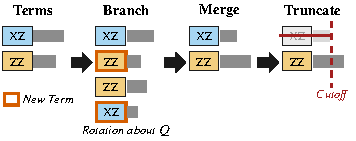
\includegraphics[scale=0.95]{figures/ops.pdf}}\hfill
\subfloat[Kicked Ising value]{\panel{bg_accuracy_a}}\hfill
\subfloat[30-qubit TFIM error]{\panel{bg_accuracy_b}}
\caption{Operations and accuracy of Pauli propagation}
\label{fig:pp}
\end{figure}

\subsection{Challenges in Distributed Pauli Propagation}
Distributed propagation must combine contributions across partitions before truncation and provide sufficient memory for intermediate expansion.
We examine these requirements in \cuPP~v0.5.0 using the 127-qubit kicked Ising circuit on NVIDIA A100 GPUs.

\noindent\textbf{Global Step after Every Gate.}
\cuPP performs a distributed merge after every gate because contributions to an identical string may reside on different GPUs.
Each MPI rank applies the gate to its local terms and issues 22 allgather calls during merge and redistribution in the measured trace.
These collectives occur even though 57\% of the gates exchange no terms.
This global step adds a fixed cost of 5.9, 22.5, and 29.8~ms per gate on 4, 8, and 16 GPUs, against 0.05-0.8~ms on one GPU (Figure~\ref{fig:anatomy}).
The measured workload reaches 22.5 million intermediate terms and takes 2.9-3.2~s on one GPU, compared with 33-48, 65, and 71~s on 4, 8, and 16 GPUs.
GPU computation occupies 9\% of execution time in this trace.
The largest rank holds 1.001 times the mean term count, indicating nearly uniform term distribution.
The increasing gate-level coordination cost limits performance despite this balance.

\noindent\textbf{Capacity Bound by the GPU Memory.}
\cuPP stores each rank's expansion and execution workspace in GPU memory.
Across the seven circuits, intermediate term counts reach 2.9-36 times the population at the start of a gate group.
Merge workspace requires additional memory alongside these intermediate terms.
\cuPP exhausts memory at 88-104 million retained terms per rank on 1-16 GPUs, although the retained payload occupies only about 4~GB of the 36~GB device-memory budget.
Deferred deduplication reduces merge frequency, but duplicate strings exhaust the memory of 16 GPUs in two of the seven circuits.
Without the global merge, local truncation also changes the expectation value to 0.1675 on four GPUs and 0.189 on 16 GPUs, compared with the merged value of 0.1531.
Available storage must accommodate intermediate expansion and workspace while preserving the merge required for coefficient truncation.

\begin{figure}[t]
\centering
\subfloat[Run time]{\panel{bg_time_a}}\hfill
\subfloat[Fixed cost per gate]{\panel{bg_gatecost_a}}\hfill
\subfloat[Terms per GPU at failure]{\panel{bg_capacity_a}}
\caption{Distributed mode of \cuPP}
\label{fig:anatomy}
\end{figure}

\subsection{Opportunity in Parities Conserved by Windows}
A partition conserved across several gates can permit local merge and truncation throughout those gates.
We examine the available conserved parities in seven circuits and their distribution over kicked Ising terms.

\noindent\textbf{Parities Conserved by Windows of Gates.}
A rotation with generator $Q$ can produce the string $P\oplus Q$ from $P$.
Every row $r$ satisfying $r\cdot Q=0$ assigns the same parity to both strings.
A window of consecutive gates conserves rows orthogonal to all its generators, permitting independent propagation within the resulting sectors.
Table~\ref{tab:windows} counts windows under a rule that retains at least $n$ independent conserved rows for an $n$-qubit circuit.
The seven circuits contain 1,100-7,960 gates and form 8-45 windows, reducing potential term-exchange boundaries by factors of 89-398 relative to gate boundaries.
The full circuits conserve at most two independent parities in this analysis, and their live terms have identical values on those parities.
Full-circuit conserved rows consequently cannot divide the measured expansions, whereas window-specific rows provide nontrivial partitions.

\noindent\textbf{Communication with Fixed Partitions.}
The linear partition in paulistrings-rs retains fixed rows throughout propagation~\cite{paulistrings}.
In the following analysis, gates act directly on strings without a Clifford frame.
A generator that changes a partition label requires inter-partition communication when the affected terms are present.
With 16 parts, random rows over all bits permit label changes at 93-96\% of the gates in the seven circuits, compared with 31-95\% for rows restricted to x bits or z bits.
On the kicked Ising circuit, random rows change the owner of 94\% of the terms at a layer of two-qubit gates, and rows over lattice regions reduce this share to 68-89\% with the largest of 16 parts at 1.65-3.37 times the mean.
The implementation lists automatic row selection as an open problem~\cite{paulistrings}.
A row change requires repartitioning the retained strings, making both its frequency and the resulting load balance relevant to execution cost.

\begin{table}[t]
\caption{Window counts and fixed-partition communication in seven circuits}
\label{tab:windows}
\centering
\small
\begin{tabular}{@{}lrrrrr@{}}
\toprule
\textbf{Circuit} & \textbf{Gates} & \textbf{Windows} & \makecell[r]{\textbf{Gates per}\\\textbf{Window}} & \makecell[r]{\textbf{Moving Gates}\\\textbf{(Random Rows)}} & \makecell[r]{\textbf{Moving Gates}\\\textbf{(z Rows)}} \\
\midrule
Kicked Ising & 5,420 & 20 & 271 & 94\% & 50\% \\
TFIM heavy-hex & 5,420 & 45 & 120 & 93\% & 50\% \\
Noisy kicked Ising & 7,960 & 20 & 398 & 95\% & 50\% \\
TFIM 11$\times$11 & 3,410 & 24 & 142 & 94\% & 60\% \\
XXZ 8$\times$8 & 2,048 & 23 & 89 & 94\% & 62\% \\
QAOA & 1,100 & 8 & 138 & 94\% & 60\% \\
Ansatz & 4,784 & 34 & 141 & 96\% & 95\% \\
\bottomrule
\end{tabular}
\end{table}

\noindent\textbf{Partition Selection from Live Terms.}
Window generators determine valid rows, while the distribution of live strings determines the population of each sector.
For kicked Ising at cutoff $10^{-5}$, the population at window starts increases from one to 159 million terms (Figure~\ref{fig:windows}).
Early windows have insufficient terms to occupy all GPUs, whereas later windows require multiple sectors per node.
Intermediate growth further changes sector sizes within a window.
A row set that balances one boundary population need not balance the population at another boundary, even when it remains algebraically valid.
The system can use the live distribution to select rows and sector counts subject to the conservation constraints.
This separation between validity and load balance permits a partition that preserves merge locality while adapting execution granularity to the retained operator.

\begin{figure}[t]
\centering
\panel{bg_windows_legend}\\[-2pt]
\subfloat[Gates and windows]{\panel{bg_windows_a}}\hfill
\subfloat[Terms at window starts]{\panel{bg_window_terms_a}}
\caption{Windows of gates in seven circuits}
\label{fig:windows}
\end{figure}

The design in Section~\ref{sec:design} combines window-conserved partitions with run-time row selection and host-memory sector storage.
The partition supplies merge locality, while host storage accommodates sectors beyond the working set of an individual GPU.
